\maketitle

\section{Proofs for Section~\ref{sec:qit}}


\subsection{Proof of Proposition \ref{prop:povmprob}}
\label{sec:proof:prop:povmprob}


\proppovmprob*

\begin{proof}
	While this is a well-known result we were not able to identify a concise proof in the literature and provide therefore, for the sake of completeness, one here. To this end, we
	first show that $p(i)\geq 1$, for each $i$.
	\begin{align}
		p(i)
		=
		\Tr [ E(i) \rho ]
		% \nonumber
		% \\
		 &
		=
		\Tr [ D(i) D^*(i)  \rho ]
		% \nonumber
		\\
		 &
		=
		\Tr [ D(i)^*  \rho D(i) ]. \nonumber
	\end{align}
	Here we used the fact that $E(i)$ is PSD and factorized it into the product $D(i) D^*(i)$. Then we used the fact that the trace is invariant under cyclical shifts.
	Clearly, the matrix $ D(i)^*  \rho D(i)$ is PSD as we have for every vector $x$:
	\begin{align}
		x^* D(i)^*  \rho D(i) x = y^* \rho y \geq 0 \quad \text{with } y = Dx.
		\label{eq:def:psdPOVM}
	\end{align}
	As the trace of a PSD matrix is positive we have that $p(i)$ is a positive real number, \ie $p(i){\geq} 0$ for every $i$.

	Secondly, we show that $p(i)$ is normalized:
	\begin{align}
		\sum_{i=1}^N p(i)
		%  &
		=
		\sum_{i=1}^N \Tr [ E(i) \rho ]
		% \nonumber
		% \\
		%  &
		=
		\Tr [ \sum_{i=1}^N E(i) \rho ]
		% \nonumber
		% \\
		%  &
		{=}
		\Tr [  \rho ],
	\end{align}
	where we used Equation~\ref{eq:povm_normalized}.
	Exploiting the fact that the trace of a density matrix is $1$ gives us indeed $\sum_{i=1}^N p(i)=1$, and we can conclude that $p(i)$ is a valid probability distribution.
\end{proof}

\section{Proofs for Section \ref{sec:puncs}}

\subsection{Proof of Proposition \ref{prop:qopunital}}
\label{sec:proof:prop:qopunital}

\propqopunital*

\begin{proof}
	The (sufficient and necessary) condition that $\sum_j \kraus_j^* \kraus_j \leq \mathbb{1}$ stems from fact that we wish to bound the probability of a state $\qop (E(i))$ to be less than or equal to $1$, \cf \citep[Proof of Theorem 8.1]{nielsen2001quantum}. That is, we wish to have:
	\begin{align}
		\Tr [ \qop (E(i)) \rho] \leq 1. \label{eq:proof:unitalvalid:bound}
	\end{align}
	We will now show that for unital quantum operations this holds by construction and that the condition $\sum_j K_j^* K_j$ is implied.

	We start with the probability for the state $\sum_i E(i)=\mathbb{1}$:
	\begin{align}
		\Tr [ \qop (\mathbb{1}) \rho]
		=
		\Tr [ \sum_j \kraus_j  \mathbb{1} \kraus_j^* \rho ]
		=
		\Tr [ \sum_j \kraus_j  \kraus_j^* \rho ]
		=
		\Tr [  \rho ] =1
	\end{align}
	Alternatively, we write this also as:
	\begin{align}
		\Tr [ \qop (\mathbb{1}) \rho]
		=
		\Tr [ \sum_j \kraus_j  \mathbb{1} \kraus_j^* \rho ]
		=
		\sum_j \Tr [ \kraus_j  \mathbb{1} \kraus_j^* \rho ]
		=
		\sum_j \Tr [\gamma^* \kraus_j  \mathbb{1} \kraus_j^* \gamma ]
	\end{align}
	with $\rho=\gamma \gamma^*$.

	Similarly, we also write for the probability of the arbitrary state $\sigma$ denoting the sum over any subset of the POVM $\{ E(i) \}_{i=1}^{N}$:
	\begin{align}
		\Tr [ \qop (\sigma) \rho]
		=
		\sum_j \Tr [\gamma^* \kraus_j \sigma \kraus_j^* \gamma ].
	\end{align}
	We now need that $\Tr [ \qop (\sigma) \rho]\leq1$, which is equivalent to:
	\begin{align}
		1 - \Tr [ \qop (\sigma) \rho] \geq 0
		 & \Leftrightarrow
		\Tr [ \qop (\mathbb{1}) \rho] - \Tr [ \qop (\sigma) \rho] \geq 0
		\\
		 & \Leftrightarrow
		\sum_j \Tr [\gamma^* \kraus_j  \mathbb{1} \kraus_j^* \gamma ]
		-
		\sum_j \Tr [\gamma^* \kraus_j \sigma \kraus_j^* \gamma ] \geq 0
		\\
		 & \Leftrightarrow
		\sum_j \Tr \Bigl[\gamma^* \kraus_j  \Bigl( \mathbb{1} -\sigma \Bigr)  \kraus_j^* \gamma \Bigr] \geq 0
	\end{align}
	The last line only holds if $\mathbb{1}- \sigma$ is PSD, which is indeed the case as $\sigma$ only sums over a subset of the POVM. Subtracting the sum of this subset from $\mathbb{1}$ leaves us with a sum over the remaining elements of the POVM. As this is a sum over PSD matrices the sum over the remaining elements is again PSD.
	This concludes the proof as we have shown that Equation~\ref{eq:proof:unitalvalid:bound} is satisfied by construction.
\end{proof}




\subsection{Proof of Proposition \ref{prop:puncPOVM}}
\label{sec:proof:prop:puncPOVM}

\proppuncPOVM*

\begin{proof}
	Given that positive unital circuits are by definition positive operator circuits we already have that:
	\begin{align}
		\forall \xvars \in \Omega(\Xvars): \Ocircuit(\xvars) \text{ is PSD}.
	\end{align}
	Next we show that $\sum_{\xvars\in \Omega(\Xvars)} \Ocircuit(\xvars)=\mathbb{1}$. Here we observe that in the computation units we have:
	\begin{align}
		\sum_{\xvars_k \in \Omega(\Xvars_k)} \Ocircuit_k(\xvars_k)
		 & = \sum_{\xvars_{k_l}} \sum_{\xvars_{k_r}}    \qop(\Ocircuit_k(\xvars_{k_l}) \otimes \Ocircuit_k(\xvars_{k_r})  )
		\\
		 & =
		\qop \left(
		\sum_{\xvars_{k_l}}   \Ocircuit_k(\xvars_{k_l})
		\otimes
		\sum_{\xvars_{k_r}}\Ocircuit_k(\xvars_{k_r})
		\nonumber
		\right)
	\end{align}
	This lets us push down the summation of a specific variable to the corresponding leaf where the variable is given as input, where we then have:
	\begin{align}
		\sum_{\xvars_k \in \Omega(\Xvars_k)} \Ocircuit_k(\xvars_k)
		= \sum_{\xvar_k\in \Omega(X_k)} E_{\xvar_k}
		= \mathbb{1_k}
	\end{align}
	We now exploit that the completely positive maps in a positive unital circuit are unital, which gives us indeed
	$
		\sum_{\xvars\in \Omega(\Xvars)} \Ocircuit(\xvars)=\mathbb{1}.
	$
\end{proof}













% \subsection{Proof of Proposition \ref{prop:computationalcomplexity}}
% \label{sec:proof:prop:computationalcomplexity}

% \propcomputationalcomplexity*

% \begin{proof}
% 	We determine the computational cost of evaluating the circuit by determining the cost of the individual computation units. We start at the leaves where we first have a Kronecker product $ e_{\xvar_k} \otimes  e_{\xvar_k}^*$, which can be performed in $\bigO (\samplespacesize^2)$.
% 	The matrix products with $A_k$ and $A_k^*$ can then be performed in $\bigO (\numbond^2 \samplespacesize)$, which implies $\bigO(\bigO (\samplespacesize^2))$ if $B\leq N$.
% 	In the qop form (\cf Equation~\ref{eq:polyadicqop}) we perform four matrix-matrix product in $\bigO (\numbond^3)$. This is followed by a Hadamard product in $\bigO (\numbond^2)$,
% 	This means that we have for the individual computation units in the partition a circuit a cost of $\bigO (\samplespacesize^3)$.

% 	It is also easy to show that for binary tree partition circuits we have a total of $\bigO (\numvar)$ computation units. This results in a computational complexity of $\bigO (\numvar  \samplespacesize^3)$.

% 	We note the computation of trace of the matrix-matrix multiplication between $\Ocircuit_{root}(\xvars)$ and the density matrix $\rho$ necessary for obtaining a probability can be done in $\bigO(\numbond^2)$.

% 	Given that we can evaluate \puncs $\bigO ( \numvar \samplespacesize^3)$ and also that we can marginalize out variables by pushing the summation to the leaves (\cf the proof of Proposition~\ref{prop:puncPOVM}), we can conclude that marginal inference has complexity $\bigO(\numvar \samplespacesize^3)$, as well.
% \end{proof}





\section{Proofs for Section \ref{sec:special_cases}}

\subsection{Proof of Proposition \ref{prop:Oveq}}
\label{sec:proof:prop:Oveq}


\propOveq*

\begin{proof}
	We start the proof at the leaf where we have
	\begin{align}
		\Ocircuit_k(\xvar_k)
		=
		U_k \left( e_{\xvar_k} \otimes e_{\xvar_k}^*  \right) U_k^*
		=
		\left( U_k e_{\xvar_k} \right) \otimes \left( e_{\xvar_k}^* U_k^* \right)
	\end{align}
	and Equation~\ref{eq:def:opvec_equivalent} holds almost by definition. In the computation units into which the leaves feed, we then have
	\begin{align}
		\Ocircuit_k
		 & = U_k \left( \Ocircuit_{k_l} \otimes \Ocircuit_{k_r} \right) U_k^*
		\nonumber
		\\
		 & = U_k \left( (\Vcircuit_{k_l} \otimes \Vcircuit^*_{k_l}) \otimes (\Vcircuit_{k_r} \otimes \Vcircuit^*_{k_r} ) \right) U_k^*
		\nonumber
		\\
		 & = \Bigl( U_k \left( \Vcircuit_{k_l} \otimes \Vcircuit_{k_r} \right) \Bigr)
		\otimes
		\Bigl( \left( \Vcircuit^*_{k_l}  \otimes \Vcircuit^*_{k_r}  \right) U_k^* \Bigr)
		\nonumber
		\\
		 & = v_k \otimes v_k^*.
	\end{align}
	where we omitted the explicit dependencies on the variables $\xvar_k$, $\xvar_{k_l}$, and $\xvar_{k_r}$.
	Repeating this argument recursively until the root of the circuit concludes the proof.
\end{proof}





\subsection{Proof of Proposition \ref{prop:voequiprob}}
\label{sec:proof:prop:voequiprob}

\propvoequiprob*





\begin{proof}
	The proof starts by simply plugging in the vector representation of $\Ocircuit_{\text{root}}$ (obtained in the proof of Proposition~\ref{prop:Oveq}) into the expression $\Tr [\Ocircuit_{\text{root}} \rho]$ and rather straightforwardly get:
	\begin{align}
		\Tr [\Ocircuit_{\text{root}} \rho]
		 &
		=
		\Tr \left[
			\Bigl(\Vcircuit_{\text{root}} \otimes \Vcircuit^*_{\text{root}}   \Bigr) \times \rho
			\right]
		\\
		 & = \Vcircuit^*_{\text{root}} \times  \rho \times\Vcircuit_{\text{root}},
	\end{align}
	which is indeed the same probability as defined in Definition~\ref{def:vpoc}.
\end{proof}


















\subsection{Proof of Proposition \ref{prop:circuit_is_prob}}
\label{app:circuit_is_prob}

\proplpcvalid*

\begin{proof}
	If $\Pcircuit_{root} (\xvars)$ is the computation unit at the root of the layered PC, each entry $i$ of $\Pcircuit_{root} (\xvars)$ forms a probability distribution if $\forall i: \Pcircuit_{root, i}(\xvars)\geq 0$, for every $\xvars \in \Omega(\Xvars)$ and if $\forall i: \sum_{\xvars \in \Omega(\Xvars)} \Pcircuit_{root, i}(\xvars)=1$. The first condition is trivially satisfied as the circuit only performs linear operations on matrices and vectors ($P_{\xvar_k}, W_k$) with positive entries only.
	For the condition $\sum_{\xvars \in \Omega(\Xvars)} \Pcircuit_{root}(\xvars)=1$ we observe that we can simply push down the summation for each variable to the respective leaf unit. This yields the following summation in the leaves:
	\begin{align}
		\sum_{\xvar_k \in \Omega(\Xvar_k)} W_k \times P_{\xvar_k}
		=
		W_k \times \sum_{\xvar_k \in \Omega(\Xvar_k)} P_{\xvar_k}
		=
		W_k \times \eta_{k} = \eta_{k}.
	\end{align}
	Here $\eta$ denotes a vector having as entries only ones (with appropriate dimensions). For the last step in the equation above we exploited the fact that the weight matrices $W_k$ are row-normalized.

	Passing on the marginalized leaves to the parent units gives us:
	\begin{align}
		W_k \times \Bigl( \eta_{k_l} \otimes \eta_{k_r} \Bigr)
		=
		W_k \times \eta_{k}  =  \eta_k
	\end{align}
	Repeating this process until we reach the root will eventually result in $\sum_{\xvars \in \Omega(\Xvars)} \Pcircuit_{root}(\xvars)=\eta_{root}$. This means that all the entries of all the vectors $\pcircuit_k(\xvars_k)$ equal to $1$ when marginalized, which means in turn that the second condition is satisfied.
\end{proof}





\subsection{Proof of Proposition \ref{prop:diagpunc}}
\label{sec:proof:prop:diagpunc}


\propdiagpunc*


\begin{proof}
	The proof is relatively straightforward as in the leaves we already have diagonal matrices by definition. For an internal unit $k$ we have that
	\begin{align}
		\Ocircuit_k = \sum_j J_j D_{kj} \left(\Ocircuit_{kl}\otimes \Ocircuit_{kr} \right)  D_{kj}^* J_j^*{kj},
	\end{align}
	which can be written as
	\begin{align}
		\Ocircuit_k = \sum_j J_j D_{kj} J_j^*{kj},
	\end{align}
	where $D_{kj}$ is diagonal and PSD. Carrying out the remaining matrix products then gives us:
	\begin{align}
		\Ocircuit_k = \sum_j H_j \Tr [D_{kj}],
	\end{align}
	which is clearly a diagonal matrix (and also PSD).
\end{proof}



\subsection{Proof of Proposition \ref{prop:PCPunciso}}
\label{sec:proof:prop:PCPunciso}


\propPCPunciso*

\begin{proof}
	In order to show this we need to show that each computation unit in a probabilistic circuit can be mapped to a computation unit in a diagonal \punc -- and vice versa. Starting at the leaves for both circuits we have
	\begin{align}
		P_{\xvar_k}
	\end{align}
	for the probabilistic circuit and
	\begin{align}
		\Delta_{\xvar_k}  \Delta_{\xvar_k}^*,
	\end{align}
	for the diagonal \punc. Given that $\Delta_{x_k}$ is a diagonal matrix the product $\Delta_{\xvar_k}  \Delta_{\xvar_k}^*$ is also a diagonal matrix with positive entries only. Taking into consideration the completeness constraints $\sum_{x_k} P_{x_k} = \eta_k $ ($\eta$ being a vector with only ones) and $\sum_{x_k} \Delta_{x_k} \Delta_{x_k}^* = \mathbb{1} $ is trivial to see that in the leaves probabilistic circuits can be mapped onto diagonal \puncs and vice versa.

	For the internal computation units we need to show that
	\begin{align}
		\phantom{\Leftrightarrow} &
		\Pcircuit_k
		=
		W_k {\times} \Bigl(\Pcircuit_{k_l} {\otimes} \Pcircuit_{k_r}\Bigr)
		\\
		\Leftrightarrow           &
		\Pcircuit_{ki}
		=
		\sum_j W_{kij} {\times} \Bigl(\Pcircuit_{k_l} {\otimes} \Pcircuit_{k_r}\Bigr)_j
		\label{eq:proof:iso:vecunit}
	\end{align}
	is equivalent to
	\begin{align}
		\Ocircuit_k = \qop (\Ocircuit_{k_l} \otimes \Ocircuit_{k_r})
		=
		\sum_j J_j D_{kj} (\Ocircuit_{k_l} \otimes \Ocircuit_{k_r}) D^*_{kj} J_j^*.
		\label{eq:proof:iso:sumdiag}
	\end{align}
	We first note that for diagonal \puncs all the operators $\Ocircuit_k$ are representable as diagonal matrices. This allows us to rewrite Equation~\ref{eq:proof:iso:sumdiag} as
	\begin{align}
		\Ocircuit_k = \qop (\Ocircuit_{k_l} \otimes \Ocircuit_{k_r})
		=
		\sum_j  J_j  \underbrace{ D_{kj} D^*_{kj}}_{\eqqcolon \Lambda_{kj}} (\Ocircuit_{k_l} \otimes \Ocircuit_{k_r})  J_j^*.
	\end{align}
	When writing out this sum of matrix product on the right-hand side explicitly it is trivial to observe that the diagonal element $\Ocircuit_{kjj}$ can be written as:
	\begin{align}
		\Ocircuit_{kjj}
		=
		\Tr \left[  \Lambda_{kj} \times (\Ocircuit_{k_l} \otimes \Ocircuit_{k_r}) \right],
	\end{align}
	with all the off-diagonal elements being zero. This can in turn be written as
	\begin{align}
		\Ocircuit_{kjj}
		=
		\sum_i  \diagvec ( \Lambda_{kj} )_i  \Bigl( \diagvec (\Ocircuit_{k_l}) \otimes \diagvec (\Ocircuit_{k_r}) \Bigr)_i,
	\end{align}
	where $\diagvec (\Lambda_{kj})$ denotes a vector whose entries corresponds to the diagonal elements of $\Lambda_{kj}$.

	Switching around the names of the indices $i$ and $j$ we can write:
	\begin{align}
		\diagvec (\Ocircuit_{k} )_i
		=
		\sum_j  \diagvec ( \Lambda_{ki} )_j  \Bigl( \diagvec (\Ocircuit_{k_l}) \otimes \diagvec (\Ocircuit_{k_r}) \Bigr)_j.
		\label{eq:proof:iso:opunit}
	\end{align}
	We now identify the expressions in Equation~\ref{eq:proof:iso:vecunit} and Equation~\ref{eq:proof:iso:opunit} as follows with each other:
	\begin{align}
		\diagvec (\Ocircuit_{k} )_i   & = \Pcircuit_{ki}
		\\
		\diagvec (\Lambda_{ki} )_j    & = W_{kij}
		\\
		\diagvec (\Ocircuit_{k_l} )_i & = \Pcircuit_{k_l i}
		\\
		\diagvec (\Ocircuit_{k_r} )_i & = \Pcircuit_{k_r i}.
	\end{align}
	This -- together with the equivalence between $\forall k: \Tr [D_{ki}D^{*}_{ki}]= \Tr [\Lambda_{ki}] =1$ and the row-normalization of the $W_k$'s -- establishes the isomorphism between the two circuit classes.
\end{proof}


% \subsection{Proof of Proposition \ref{prop:computationalcomplexityvec}}
% \label{sec:proof:prop:computationalcomplexityvec}


% \propcomputationalcomplexityvec*

% \begin{proof}
% 	Following a similar train of thought as the proof in Section~\ref{sec:proof:prop:computationalcomplexity} we can derive the computational cost of evaluating a positive vector circuit to be $\bigO (\numvar \numbond \samplespacesize)$ implying
% 	$\bigO (\numvar  \samplespacesize^2)$
% 	when $\numbond \leq \samplespacesize$.
% 	The major difference between matrix representation of operator circuits and their vector representation is that for the former the internal computation units output matrices ($\Ocircuit_k(\xvars_k)\in \mathbb{C}^{\numbond \times \numbond}$) while for the latter vectors are outputted ($\Vcircuit_k(\xvars_k)\in \mathbb{C}^{\numbond}$).



% 	As $\Vcircuit_{root}(\Xvar_{rooot})$ is computable in $\bigO (\numvar \numbond \samplespacesize)$ and $\lVert \gamma \times \Vcircuit_{\text{root}}\rVert^2$ is computable in $\bigO(\numbond^2)$, we can conclude that the probability $p_\Xvars(\xvars)$ can be computed in $\bigO (\numvar \samplespacesize^2)$.
% \end{proof}







\section{Noisy and Block-Diagonal \puncs}
\label{sec:noisyblockdiagonalpuncs}

In order to increase the expressive power of non-monotone circuits, \citet{loconte2025sum} proposed to multiply a pure \punc with a probabilistic circuit.
This was motivated by their observation that the expressive power of monotone and squared circuits (a special case of pure \puncs) are incomparable \citep{decolnet2021compilation}. That is, each of these circuit classes can express circuits that would lead to an exponential blow-up in the respective other circuit class. The idea is relatively simple: they express an unnormalized probability distribution as the product of a probabilistic circuit and a traced \punc:
\begin{align}
	\qcircuit(\xvars) \Tr [\Ocircuit(\xvars) \rho].
\end{align}
They called such a model a \msocs. We will put these models in a quantum information theoretic framework. This will then lead to the realization that \msocss are nothing but block-diagonal operator circuits.


\subsection{Sub-Complete Probability Distributions}

An important concept in quantum information theory that generalizes the standard POVM (\cf Definition~\ref{def:povm}) is the so-called noisy POVM, which enables for instance modelling imperfect measurement devices. In the context of machine learning this might be an improperly labeled data point of an error in the detector, \eg a pixel flip in the camera that took a picture.
\begin{definition}
	\label{def:noisypovm}
	A noisy positive operator-valued measure
	is a set of PSD  matrices $\{E(i)\}_{i=0}^{I-1}$ ($\numevents$ being the number of possible measurement outcomes) such that:
	\begin{talign}
		\sum_{i=0}^{I-1} E(i) = \subcompletemeasrure < \mathbb{1},
	\end{talign}
	where the inequality sign is interpreted using the Loewner ordering of PSD matrices,
	\ie $\subcompletemeasrure < \mathbb{1} \Leftrightarrow\mathbb{1}-\subcompletemeasrure$ is PSD.
\end{definition}

\begin{definition}[Sub-complete Probability Distribution]
	Let $\Xvars$ be a set of random variables with sample space $\Omega(\Xvars)$. We call a probability distribution \textit{sub-complete} if $\forall \xvars \in \Omega(\Xvars): p(\xvars)\geq 0$ and if $\sum_{\xvars \in \Omega(\Xvars)} p(\xvars)\leq 1$. We call a probability distribution \textit{strictly sub-complete} if the latter inequality holds strictly and \textit{complete} if equality holds.
\end{definition}




\begin{restatable}{proposition}{propnoisypovmdist}
	\label{prop:noisypovmdist}
	Noisy POVMs induce a sub-complete probability distributions.
\end{restatable}

\begin{proof}
	Let $\rho$ be a density matrix and $\{E(i)\}_{i=0}^{I-1} $ be a POVM such that $\sum_{i=0}^{I-1} E(i)=M$. We then have
	\begin{align}
		\Tr[(\mathbb{1}-M) \rho]\geq 0,
	\end{align}
	holds as $\mathbb{1}-M$ is PSD by definition.
	Pushing the trace over the subtraction and rearranging terms yields:
	\begin{align}
		\Tr[\mathbb{1} \rho]- 	\Tr[M \rho]\geq 0 \Leftrightarrow \Tr[M \rho]\leq 1.
	\end{align}
	This means that the induced probability distribution $p(i)= \Tr[E(i)\rho]$ is indeed sub-complete.
\end{proof}






To construct sub-complete probability distributions using operator circuits we now introduce \textit{noisy positive unital circuits} or \noisepuncs.

\begin{definition}
	\label{def:noisepunc}
	A \noisepunc $\Qcircuit(\xvars)$ is of the form
	\begin{align}
		\Qcircuit(\xvars)= \qcircuit(\xvars) \Ocircuit(\xvars),
	\end{align}
	where $\Ocircuit(\xvars)$ is a \punc and $\qcircuit(\xvars)$ is real-valued and belongs to the  $[0,1]$ interval for every $\xvars$.
\end{definition}



\begin{restatable}{proposition}{propnoisepunddist}
	\label{prop:noisepunddist}
	\noisepuncs induce sub-complete probability distributions.
\end{restatable}

\begin{proof}
	Let $\Xvars$ be a set of random variables and  $\Qcircuit(\xvars)= \qcircuit(\xvars)\Ocircuit(\xvars)$ with $\xvars\in \Omega(\Xvars)$ be a \noisepunc inducing a probability distribution
	\begin{align}
		\pi_\Xvars(\xvars) = \Tr [ \qcircuit(\xvars)\Ocircuit(\xvars) \rho].
	\end{align}
	As $\qcircuit(\xvars)$ is a scalar we can write
	\begin{align}
		\pi_\Xvars(\xvars) = \qcircuit(\xvars) \Tr [ \Ocircuit(\xvars) \rho] = \qcircuit(\xvars) p_X(\xvars),
	\end{align}
	where $p_X(\xvars)$ is the (complete) probability distribution induced by the set $\{ \Ocircuit(\xvars) \}_{\xvars \in \Omega(\Xvars)}$. As $0\leq q(\xvars)\leq 1$ (by definition) and $0\leq p_\Xvars(\xvars)\leq 1$ we have also that $0\leq \pi_\Xvars(\xvars)\leq 1$. This shows that each event $\xvars\in \Omega(\Xvars)$ has a positive probability.

	For the sub-completeness we observe that the sum of positive terms
	\begin{align}
		\sum_{\xvars \in \Omega(\Xvars)} p_\Xvars(\xvars)=1.
	\end{align}
	If we weigh each term in the sum with a scalar $q(\xvars) \in [0,1]$ we immediately conclude that $\sum_{\xvars \in \Omega(\Xvars)} \pi_\Xvars (\xvars)\leq$ and that we have indeed a sub-complete probability distribution.
\end{proof}



\subsection{Noise Variables}


All of this is a bit unnerving. How is it possible that we have probabilistic events $\xvars\in \Omega(\Xvars)$ that violate the second of Kolmogorov's probability axioms (by having sub-complete distributions)? The resolution to this problem lies in interpreting sub-complete distributions as joint distributions not only over the set of variables $\Xvars$ but an extra set of variables $\Yvars$ representing extra noise~\citep{wiseman2009quantum}
\begin{align}
	\pi_{\Xvars}(\xvars) = p_{\Xvars \Yvars}(\xvars, \yvars),
\end{align}
for which we indeed have
\begin{align}
	\sum_{\xvars\in \Omega(\Xvars)} \sum_{\yvars\in \Omega(\Yvars)}  p_{\Xvars \Yvars}(\xvars, \yvars) =1.
\end{align}
The problem with the random variables $\Yvars$ is that they are not accessible to the observer. In the sense that they are observable in principle but in practice not, \eg a defect in a sensor.\footnote{Note these practically unobservable variables should not be confused with the concept of (local) hidden variables, which lead to violations of Bell's inequality.}
However, the probability we are actually interested in is the one for $\Xvars$ given $\Yvars$
\begin{align}
	p_{\Xvars|\Yvars}(\xvars\mid \yvars )
	 & =
	\frac{
	p_{\Xvars \Yvars}(\xvars,  \yvars )
	}
	{
	\sum_{\xvars\in \Omega(\Xvars)}p_{\Xvars \Yvars}(\xvars, \yvars )
	}
	\nonumber
	\\
	 & = \frac{\pi_{\Xvars}(\xvars)}{\sum_{\xvars\in \Omega(\Xvars)}  \pi_{\Xvars}(\xvars)}
\end{align}
The question now became whether we can choose $\qcircuit(\xvars)$ such that the summation in the denominator is tractable, \ie can be performed in time polynomial in the number of random variables $\Xvars$.


In the probabilistic circuit literature it has been shown that the product of two circuits is representable as a single circuit within polytime and polyspace if the two circuits are compatible~\citep{khosravi2019tractable,vergari2021compositional}. Importantly, this single circuit then allows for summing out the variables $\xvars$.
As pointed out also by \citet{loconte2025sum}, all we need is that $\qcircuit(\xvars)$ and $\Ocircuit(\xvars)$ are both structured decomposable according to the same partition tree (or variable tree). Furthermore, we pick $\qcircuit(\xvars)$ to be a probabilistic circuit and $\Ocircuit(\xvars)$ to be a \punc.
For the sake of simplicity we construct the circuit $\qcircuit(\xvars)$ (with an underlying partition circuit) using
Hadamard products instead of Kronecker products.
\begin{align}
	{\qcircuit}_k(\xvars_k)=
	\begin{cases}
		f_{\xvar_k},
		 & \text{if $k$ leaf}
		\\
		W_k \times \Bigl( \qcircuit_{k_l}(\xvars_{k_l}) \odot  \qcircuit_{k_r} (\xvars_{k_r}) \Bigr)
		 & \text{else}.
	\end{cases}
	\nonumber
\end{align}










\subsection{\noisepuncs as Deep Operator Mixtures}

An interesting consequence of modelling noise in the system via a probabilistic circuit $\qcircuit(\xvars)$ is that it effectively results in a model that can be interpreted as a recursive mixture of positive operators. To see this, let us first write the matrix vector product in the computation units of $\qcircuit(\xvars)$ using explicit indices:
\begin{talign}
	\qcircuit_k
	= W_k \times (\qcircuit_{k_l} \odot \qcircuit_{k_r})
	\Leftrightarrow  \qcircuit_{ki} = \sum_j w_{kij}  \qcircuit_{k_l j}  \qcircuit_{k_r j}.
\end{talign}
Here $\qcircuit_{ki}$ denotes the $i$-th entry of the vector $\qcircuit_{k}$ and $w_{kij}$ denotes the elements of the matrix $W_k$.
We also dropped the explicit dependency on $\xvars_k$.

We now multiply each $\qcircuit_{ki}\in [0,1]$ with the corresponding operator $\Ocircuit_k$
\begin{talign}
	\qcircuit_{ki} \Ocircuit_k
	& = \left(\sum_j w_{kij}  \qcircuit_{k_l j}  \qcircuit_{k_r j} \right)  \qop_k( \Ocircuit_{k_l} \otimes \Ocircuit_{k_r} )
	\nonumber
	\\
	& =\sum_j w_{kij}  \underbrace{\qop_k(  \qcircuit_{k_l j} \Ocircuit_{k_l} \otimes  \qcircuit_{k_r j} \Ocircuit_{k_r} )}_{=\tildeQcircuit_{kj}}
	\label{eq:deepoperatirmix}
\end{talign}
This means that we have for each computation unit $k$ not one but multiple operators, indexed by $i$, and each of the  $i$ operators is a mixture of operators:
\begin{talign}
	\Qcircuit_{ki}(\xvars_k) =\sum_j w_{kij} \tildeQcircuit_{kj}(\xvars_k).
	\label{eq:operatormix}
\end{talign}
We illustrate the situation in Figure~\ref{fig:operatormixture}. Such mixtures of operators can be regarded as generalizing standard mixture models of probability distributions, which can be recovered by considering the special case of operators of dimension one -- in other words positive real-valued scalars. With this interpretation we can follow a similar reasoning to viewing probabilistic circuits as \puncs closed over diagonal matrices. But now we view \noisepuncs as \puncs closed over block-diagonal matrices.

\begin{figure}[t]
	\centering
	\resizebox{0.7\columnwidth}{!}{
	\centering




	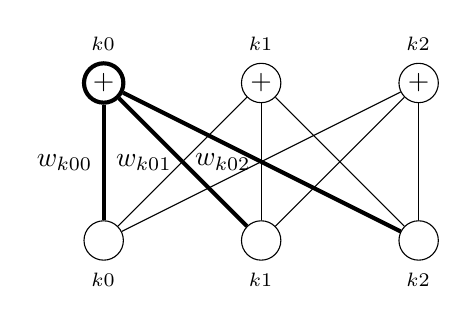
\begin{tikzpicture}[node distance=2cm, auto]

		% Upper layer nodes with increased size
		\node[draw, circle, minimum size=0.5cm,inner sep=1pt, line width=1.5pt] (A1) at (0, 2) {$+$};
		\node[draw, circle, minimum size=0.5cm,inner sep=1pt] (A2) at (2, 2) {$+$};
		\node[draw, circle, minimum size=0.5cm,inner sep=1pt] (A3) at (4, 2) {$+$};
		% Lower layer nodes with increase size
		\node[draw, circle, minimum size=0.5cm] (B1) at (0, 0) {};
		\node[draw, circle, minimum size=0.5cm] (B2) at (2, 0) {};
		\node[draw, circle, minimum size=0.5cm] (B3) at (4, 0) {};

		% Labels for the upper layer
		\node at (0, 2.5) {$\Qcircuit_{k0}$};
		\node at (2, 2.5) {$\Qcircuit_{k1}$};
		\node at (4, 2.5) {$\Qcircuit_{k2}$};

		% Labels for the lower layer
		\node at (0, -0.5) {$\tildeQcircuit_{k0}$};
		\node at (2, -0.5) {$\tildeQcircuit_{k1}$};
		\node at (4, -0.5) {$\tildeQcircuit_{k2}$};

		% Connecting upper layer to lower layer
		\foreach \i in {1,2,3}{
				\foreach \j in {1,2,3}{
						\draw (A\i) -- (B\j);
					}
			}



		% Thicker edges connected to the upper-left node
		\draw[line width=1.5pt] (A1) -- (B1) node[midway, left]{$w_{k00}$};
		\draw[line width=1.5pt] (A1) -- (B2) node[midway, left] {$w_{k01}$};
		\draw[line width=1.5pt] (A1) -- (B3) node[midway, left] {$w_{k02}$};

	\end{tikzpicture}
}
	\caption{
	Graphical representation of operator mixing as described in Equation~\ref{eq:operatormix}. The operators $\Qcircuit_{k0}$, $\Qcircuit_{k1}$, and $\Qcircuit_{k2}$ are all PSD matrices and constructed using the operators  $\tildeQcircuit_{k0}$, $\tildeQcircuit_{k1}$, and $\tildeQcircuit_{k2}$ using weighted sums. For $\Qcircuit_{k0}$ we also indicate the mixing weights $w_{k00}$, $w_{k01}$, and $w_{k02}$, which are positive real-valued scalars and satisfy $w_{k00}+ w_{k01}+w_{k02}=1$.
	}
	\label{fig:operatormixture}
\end{figure}





\section{Proofs for Section \ref{sec:nsdnmcircuit}}



\subsection{Proof for Theorem \ref{theo:properprobdpunc}}
\label{sec:proof:theo:properpropdpunc}

\theoproperprobdpunc*

\begin{proof}
	The proof is relatively straightforward as positivity is guaranteed by the fact that we perform computations on members of POVMs that all preserve positive semi-deifiniteness (Kronecker product in the product units and convex combination of quantum operations in the sum units). This guarantees that $\ocircuit(\xvars)$ is PSD and hence $ \Tr [\ocircuit(\xvars) \rho]>0$. The argument is similar for the completeness of $\Tr [\ocircuit(\xvars) \rho]$ as here we need to show that $\sum_{\xvars \in \Omega(\Xvars)} \ocircuit(\xvars) =\mathbb{1}$. For this we push down the summations to the corresponding leaves where we obtain unit matrices. The circuit then performs again computation with these unit matrices that are all unital, which guarantees indeed that
	\begin{align}
		\sum_{\xvars \in \Omega(\Xvars)} \Tr [\ocircuit(\xvars) \rho]
		 & =
		\Tr \left[
			\left(
			\sum_{\xvars \in \Omega(\Xvars)}\ocircuit(\xvars)
			\right)
			\rho
			\right]
		\\
		 & =
		\Tr \left[  \mathbb{1} \rho\right]
		\nonumber
		\\
		 & =1
		\nonumber
	\end{align}
\end{proof}



\subsection{Proof of Proposition \ref{prop:sdpuncsubsetdpunc}}
\label{sec:proof:prop:sdpuncsubsetdpunc}

\propsdpuncsubsetdpunc*


\begin{proof}
	Consider the expression of a sum unit in a \dpunc
	\begin{align}
		\sum_{j\in\inputs(k)} \weight_{kj} \qop_{kj} (\ocircuit_j(\xvars_j) ).
	\end{align}
	Writing also the operation that is performed in the product units we obtain:
	\begin{align}
		\sum_{j\in\inputs(k)} \weight_{kj} \qop_{kj} \Bigl(\ocircuit_{j_l}(\xvars_{j_l}) \otimes \ocircuit_{j_r}(\xvars_{j_r})   \Bigr).
	\end{align}
	Given that all product units decompose in the same way we can write this as
	\begin{align}
		\sum_{j\in\inputs(k)} \weight_{kj} \qop_{kj} \Bigl(\ocircuit_{j_l}(\xvars_{k_l}) \otimes \ocircuit_{j_r}(\xvars_{k_r})   \Bigr),
	\end{align}
	where the index on $\xvars_j$, $\xvars_{j_l}$, and $\xvars_{j_r}$ is now on $k$ and not on $j$. Given that the expression above is a completely positive map \citep{nielsen2001quantum} that maps positive semi-definite matrices to positive semi-definite matrices, we can write the expression using a single quantum operation:
	\begin{align}
		\qop_{k} \Bigl(\ocircuit_{k_l}(\xvars_{k_l}) \otimes \ocircuit_{k_r}(\xvars_{k_r})   \Bigr).
	\end{align}
	Following the convention from Section~\ref{sec:puncs} and using upper case letter for the circuit we have:
	\begin{align}
		\qop_{k} \Bigl(\Ocircuit_{k_l}(\xvars_{k_l}) \otimes \Ocircuit_{k_r}(\xvars_{k_r})   \Bigr),
	\end{align}
	which corresponds exactly to the computations performed in an \sdpunc and thereby concludes the proof.
\end{proof}










% \subsection{Normalizing Positive Operator Circuits}

% Using \noisepuncs instead of \puncs we run into the issue of not having a normalized probability distribution anymore. One possibility would be to compute an overall normalization constant as done, for instance in \citep{loconte2025sum} and \citep{wangrelationship}. However, we can be more ambitous and turn non-unital computation units in \sdpunc into unital ones. For this, consider the non-untial computation unit
% \begin{align}
% 	\Ocircuit_k(\xvars_k) =\sum_i \kraus_{ki} (\Ocircuit_{k_l}(\xvars_{k_l}) \otimes \Ocircuit_{k_r}(\xvars_{k_r})) \kraus_{ki}^*
% \end{align}
% Marginalizing on both sides we obtain:
% \begin{align}
% 	 & \phantom{\Leftrightarrow} \sum_{\xvars_k}\Ocircuit_k(\xvars_k)
% 	=\sum_i \kraus_{ki}
% 	\left(  \sum_{\xvars_{k_l}}(\Ocircuit_{k_l}(\xvars_{k_l}) \right)
% 	\otimes
% 	\left(\sum_{\xvars_{k_r}}\Ocircuit_{k_r}(\xvars_{k_r}))  \right)
% 	\kraus_{ki}^*
% 	\\
% 	 & \Leftrightarrow
% 	R_k = \sum_i \kraus_{ki} (R_{k_l} \otimes R_{k_r}) \kraus_{ki}^*
% 	\\
% 	 & \Leftrightarrow
% 	R_k = \sum_i R_k^{\nicefrac{1}{2}} R_k^{\nicefrac{-1}{2}}  \kraus_{ki}
% 	(R_{k_l} \otimes R_{k_r})
% 	\kraus_{ki}^* R_k^{\nicefrac{-1}{2}} R_k^{\nicefrac{1}{2}}
% 	\\
% 	 & \Leftrightarrow
% 	R_k = \sum_i R_k^{\nicefrac{1}{2}}   \kraus_{ki}^{'}
% 	(R_{k_l} \otimes R_{k_r})
% 	\kraus_{ki}^{'*}  R_k^{\nicefrac{1}{2}}
% 	\\
% 	 & \Leftrightarrow
% 	R_k =  R_k^{\nicefrac{1}{2}}
% 	\underbrace{
% 		\left(
% 		\sum_i \kraus_{ki}^{'} (R_{k_l} \otimes R_{k_r}) \kraus_{ki}^{'*}
% 		\right)}_{= \mathbb{1}}
% 	R_k^{\nicefrac{1}{2}}
% \end{align}
% with $ \kraus_{ki}^{'} = R_k^{\nicefrac{-1}{2}} \kraus_{ki}$







